\documentclass[11pt, openright]{book}

    % Cover Variables
	\newcommand{\ctitle}{Traitement d'Images}
        \newcommand{\cautor}{Eva Maturana- Lucas Lescure}
		\newcommand{\ctoptitle}{Travaux Pratiques}

    % Header Variables
        \newcommand{\headRE}{\emph{\thepage}}
        \newcommand{\headLE}{\emph{\thesection. \rightmark}}
        \newcommand{\footRE}{}
        \newcommand{\footLE}{}

    % TOC Variables
        \newcommand{\toctitle}{Table of Content}
        \newcommand{\tocchapter}{Chapter}
        \newcommand{\toccount}{3}
  
    % Chapter Variables
        \newcommand{\chvar}{Chapter -}

\usepackage[a4paper, total={16cm, 22.125cm}]{geometry}

% Page Style
\usepackage[]{environ}
% Cover Page 
\usepackage{tikz}
\makeatletter
\def\parsecomma#1,#2\endparsecomma{\def\page@x{#1}\def\page@y{#2}}
\tikzdeclarecoordinatesystem{page}{
    \parsecomma#1\endparsecomma
    \pgfpointanchor{current page}{north east}
    % Save the upper right corner
    \pgf@xc=\pgf@x%
    \pgf@yc=\pgf@y%
    % save the lower left corner
    \pgfpointanchor{current page}{south west}
    \pgf@xb=\pgf@x%
    \pgf@yb=\pgf@y%
    % Transform to the correct placement
    \pgfmathparse{(\pgf@xc-\pgf@xb)/2.*\page@x+(\pgf@xc+\pgf@xb)/2.}
    \expandafter\pgf@x\expandafter=\pgfmathresult pt
    \pgfmathparse{(\pgf@yc-\pgf@yb)/2.*\page@y+(\pgf@yc+\pgf@yb)/2.}
    \expandafter\pgf@y\expandafter=\pgfmathresult pt
}
\makeatother


% Object formatting
\usepackage[12pt]{moresize}
\usepackage[]{anyfontsize}
\usepackage{titlesec}
\usepackage{import}
\usepackage{floatrow}
\usepackage{enumitem}
\usepackage{changepage}
\usepackage[normalem]{ulem}
\usepackage{array}
\newcommand{\ul}[1]{\underline{#1}}

\usepackage[]{chngcntr}
\usepackage{ifthen}
\ifthenelse{\figcountdepth > 1}
  {\counterwithin{figure}{section}\counterwithin{table}{section}}
  {}

\usepackage[format=plain, labelfont=it, textfont=it]{caption}
\makeatletter
\def\@makecaption#1#2{%
    \vskip\abovecaptionskip
    \sbox\@tempboxa{\textit{#1.} #2}

       
   

    \ifdim \wd\@tempboxa >\hsize
        #1. #2\par
    \else
        \global \@minipagefalse
        \hb@xt@\hsize{\hfil\box\@tempboxa\hfil}
    \fi
    \vskip\belowcaptionskip}
\makeatother

\DeclareCaptionFormat{underline}{\uline{#1#2#3}\par}

% Sections
\titleformat{\section}{\fontsize{16}{19.2}\bfseries}{\thesection.}{0.25em}{}
\titleformat{\subsection}{\fontsize{14}{16.8}\bfseries}{\tab\thesubsection.}{0.25em}{}
\titleformat{\subsubsection}{\fontsize{10}{12}}{\uline{\thesubsubsection)\enspace}}{0em}{\uline}





% Geometry

% Typewritting

\setlength{\parskip}{1em}
\setlength{\parindent}{0em}


\newenvironment{items}[3][0pt]
{\def\closesep{#3}
    \vspace{#2}
    \begin{itemize}
        \setlength{\itemsep}{#1}
        \setlength{\topsep}{0pt}
        \setlength{\partopsep}{0pt}}
        {\end{itemize}
    \vspace{\closesep}}

\newenvironment{enum}[3][0pt]
{\defclosesep{#3}
    \vspace{#2}
    \begin{enumerate}
        \setlength{\itemsep}{#1}
        \setlength{\topsep}{0pt}
        \setlength{\partopsep}{0pt}}
        {\end{enumerate}
    \vspace{\closesep}}

\newenvironment{eq}[2]
{\def\closesep{#2}
    \vspace{#1}
    \begin{align*}}
        {\end{align*}
    \vspace{\closesep}}

\newenvironment{lfeq}[2]
{\def\closesep{#2}
    \vspace{#1}
    \begin{flalign*}}
        {\end{flalign*}
    \vspace{\closesep}}
% List Formatting


\NewEnviron{dent}[1]{
    \vspace{-10pt}
    \begin{adjustwidth}{7mm}{}
        \uline{#1}\hspace{2mm}
        \BODY
    \end{adjustwidth}
    \vspace{-10pt}
}


\usepackage[framemethod=tikz]{mdframed}
\newcounter{count_theorem}[section]\setcounter{count_theorem}{0}
\newcommand{\thetheorem}{\arabic{count_theorem}}

\newcounter{count_exercise}[section]\setcounter{count_exercise}{0}
\newcommand{\theexercise}{\arabic{count_exercise}}


\newenvironment{theorem}[1][]{
    \refstepcounter{count_theorem}
    \mdfsetup{
        linecolor=red!30,
        innerbottommargin=10pt,
        linewidth=2pt,
        topline=false,
        bottomline=false,
        rightline=false,
        shadow=true,
        shadowsize=4.5pt,
        frametitlerule=false,
        apptotikzsetting={
                \tikzset{
                    mdfbackground/.append style={
                            left color=red!8,right color=red!3
                        }
                }
            }
    }
    \begin{mdframed}[]\relax
        \ifstrempty{#1}
        {\textbf{Theorem~\thetheorem.} }
        {\textbf{Theorem~\thetheorem.~#1} }
        }
        {\end{mdframed}\vspace{-10pt}
}

\newenvironment{note}{
    \mdfsetup{innertopmargin=5pt,
        linecolor=gray!30,
        linewidth=2pt,
        topline=false,
        bottomline=false,
        rightline=false,
        frametitleaboveskip=0pt,
        shadow=false,
        shadowsize=4pt,
        frametitlerule=false,
        apptotikzsetting={
                \tikzset{
                    mdfbackground/.append style={
                            left color=gray!8,right color=gray!3
                        }
                }
            }
    }
    \begin{mdframed}[]\relax
        \textbf{Note. }
        }
        {\end{mdframed}\vspace{-10pt}
}

\newenvironment{example}{
    \mdfsetup{innertopmargin=5pt,
        linecolor=green!30,
        linewidth=2pt,
        topline=false,
        bottomline=false,
        rightline=false,
        frametitleaboveskip=0pt,
        shadow=false,
        shadowsize=4pt,
        frametitlerule=false,
        apptotikzsetting={
                \tikzset{
                    mdfbackground/.append style={
                            left color=green!7,right color=green!2
                        },
                    mdfframetitlebackground/.append style={
                            left color=green!7,right color=green!2
                        }
                }
            }
    }
    \begin{mdframed}[]\relax
        \textbf{Example. }
        }
        {\end{mdframed}\vspace{-10pt}
}


\usetikzlibrary{calc,arrows}

\tikzset{
    excursus arrow/.style={%
            line width=2pt,
            draw=gray!40,
            rounded corners=2ex,
        },
    excursus head/.style={
            fill=white,
            font=\bfseries\sffamily,
            text=gray!80,
            anchor=base west,
        },
    excursus line/.style={%
            line width=2pt,
            draw=gray!40,
            rounded corners=2ex,
        }
}

\newenvironment{exercise}[1][]{%
    \refstepcounter{count_exercise}
    \mdfsetup{
        singleextra={
                \path let \p1=(P), \p2=(O) in (\x2,\y1) coordinate (Q);
                \path let \p1=(Q), \p2=(O) in (\x1,{(\y1-\y2)/2}) coordinate (M);
                \path [excursus line] ($(O)+(5em,0ex)$) -| (M) |- ($(Q)+(20em,0ex)$);
                \node [excursus head] at ($(Q)+(2.5em,-0.75pt)$) {\ifstrempty{#1}{Exercise \theexercise}{Exercise \theexercise:~#1}};},
        firstextra={
                \path let \p1=(P), \p2=(O) in (\x2,\y1) coordinate (Q);
                \path [excursus arrow,-to] (O) |- ($(Q)+(12em,0ex)$) .. controls +(0:16em) and +(185:6em) .. ++(23em,2ex);},
        middlelinewidth=2.5em,middlelinecolor=white,
        hidealllines=true,topline=true,
        innertopmargin=0.5ex,
        innerbottommargin=2.5ex,
        innerrightmargin=2pt,
        innerleftmargin=2ex,
        skipabove=0.87\baselineskip,
        skipbelow=0.62\baselineskip,
    }
    \begin{mdframed}[]\relax}
        {\end{mdframed}\vspace{-10pt}
}

% Functions and Data Plotting
\usepackage{subfig,wrapfig,adjustbox,multirow}


% Plotting Style
\usepackage{graphicx,pgfplots}
\usetikzlibrary{arrows}
\usetikzlibrary {patterns,patterns.meta}
\usepgfplotslibrary{fillbetween}
\pgfplotsset{compat=1.18}

\usepgfplotslibrary{units}
% Logarithmic Scale
\pgfplotsset{
    log x ticks with fixed point/.style={
            xticklabel={
                    \pgfkeys{/pgf/fpu=true}
                    \pgfmathparse{exp(\tick)}%
                    \pgfmathprintnumber[fixed relative, precision=3]{\pgfmathresult}
                    \pgfkeys{/pgf/fpu=false}
                }
        }
}


% Mathematics

% Formatting
\usepackage{amsmath}
\usepackage{esvect}
\usepackage{amsfonts}
\usepackage{tasks,environ}
\usepackage{xargs}
\usepackage{esint}
\usepackage[]{listings}


\usepackage[english]{babel}
\usepackage{amsthm}
%\newtheorem{theorem}{Theorem}
%\newtheorem{proof}{Proof}



%Custom Shortcuts
\newcommand{\eqi}{\Leftrightarrow}
\newcommand{\lr}[1]{\left( #1 \right)}
\newcommand{\limit}[1]{\displaystyle{\lim_{#1}}}
\newcommand{\tab}{\hspace*{7mm}}
\newcommand{\ds}[1]{\displaystyle{#1}}
\newcommand{\floor}[1]{\lfloor #1 \rfloor}
\newcommand{\R}{\mathbb{R}}
\newcommand{\N}{\mathbb{N}}
\newcommand{\Z}{\mathbb{Z}}
\newcommand{\C}{\mathbb{C}}
\newcommand{\K}{\mathbb{K}}
\newcommand{\F}{\mathcal{F}}
\newcommand{\M}{\mathcal{M}}
\renewcommand{\l}{\lambda}
\newcommand{\seg}[1]{\overline{\rm {#1}}}
\newcommand{\Int}{\int\limits}
\newcommand{\ex}{\tab \uline{Example :}\hspace{0.2cm} }
\newcommand{\vard}{\partial}
\newcommand{\Q}{\mathcal{Q}}
\newcommand{\Vect}{\operatorname{Vect}}
\newcommand{\rg}{\operatorname{rg}}
\renewcommand{\dim}{\operatorname{dim}}
\renewcommand{\Re}{\operatorname{Re}}
\renewcommand{\Im}{\operatorname{Im}}
\renewcommand{\P}{\mathcal{P}}
\newcommand{\blr}[1]{\left\{#1\right\}}
\newcommand{\linecenter}[1]{\par\vspace{2mm} \centerline{#1}\par\vspace{-2mm}}
\newcommand{\dd}{\textrm{d}}
\newcommand{\supp}{\operatorname{Supp}}
\renewcommand{\vec}{\overrightarrow}
\renewcommand{\epsilon}{\varepsilon}

% Matrix Configurations

\makeatletter
\renewcommand*\env@matrix[1][*\c@MaxMatrixCols c]{%
    \hskip -\arraycolsep
    \let\@ifnextchar\new@ifnextchar
    \array{#1}}
\makeatother


% Colors
\usepackage{xcolor}
\newcommand{\blu}{\color{blue}}
\newcommand{\Red}{\color{red}}
\newcommand{\blac}{\color{black}}

\newcommand{\red}[1]{\textcolor{red}{#1}}

\usepackage{xcolor,xspace}
\usepackage{breqn}


% Headings  
\usepackage[Glenn]{fncychap}
\ChNumVar{\fontsize{40}{42}}
\ChTitleVar{\Large\sc}
\ChNameVar{\Large\sc}
\setlength\headheight{14.5pt}
\renewcommand\FmN[1]{\chvar}



\usepackage{fancyhdr}
\usepackage{ragged2e}

% Header & Footers
\renewcommand{\chaptermark}[1]{\markboth{#1}{#1}}
\renewcommand{\sectionmark}[1]{
    \markright{ #1}
}
\pagestyle{fancy}
\fancyhf{}
\fancyhead[LE,RO]{\headLE}
\fancyhead[RE,LO]{\headRE}
\fancyfoot[LE,RO]{\footLE}
\fancyfoot[RE,LO]{\footRE}
\renewcommand{\headrulewidth}{0.5pt}
\fancyheadoffset{1cm}

\fancypagestyle{plain}{%
    \fancyhf{} % clear all header and footer fields
    \fancyfoot[LE, RO]{\footLE}
    \renewcommand{\headrulewidth}{0pt}
    \renewcommand{\footrulewidth}{0pt}}


\fancypagestyle{nohead}{%
    \fancyhf{} % clear all header 
    \fancyfoot[LE, RO]{\footLE}
    \fancyfoot[LO, RE]{\footRE}}

    \fancypagestyle{head}{%
    \fancyhf{} % clear all header 
    \fancyhead[LE,RO]{\headLE}
\fancyhead[RE,LO]{\headRE}
\renewcommand{\headrulewidth}{0.5pt}
\fancyheadoffset{1cm}
    }


\fancypagestyle{bib}{%
    \fancyhf{} % clear all header and footer fields
    \fancyhead[CE, CO]{}
    \fancyfoot[LE, RO]{\footLE}
    \fancyfoot[LO, RE]{Bibliographie}}

% Table of Contents

\renewcommand*\thechapter{\arabic{chapter}} %Usually Roman
\renewcommand*\thesection{\arabic{section}}
\renewcommand*\thesubsubsection{\thesubsection.\alph{subsubsection}}
\makeatletter
\@removefromreset{section}{chapter}
\makeatother


% Table of Contents

\usepackage{titletoc}
\usepackage{ erewhon,cabin}
\usepackage[linktoc=all]{hyperref}
\renewcommand*\contentsname{\centerline{\toctitle}}

\setcounter{secnumdepth}{3}
\setcounter{tocdepth}{\toccount}

\usepackage[subfigure]{tocloft}
\setlength\cftparskip{0pt}

\usepackage{etoolbox}
\makeatletter
\pretocmd{\chapter}{\addtocontents{toc}{\protect\addvspace{5\p@}}}{}{}
\pretocmd{\section}{\addtocontents{toc}{\protect\addvspace{-10\p@}}}{}{}
\pretocmd{\subsection}{\addtocontents{toc}{\protect\addvspace{1\p@}}}{}{}
\makeatother


% Chapter Style
\titlecontents{chapter}
[11em]
{\bigskip}
{\bfseries\textsc\tocchapter~\textsc\thecontentslabel : \textsc}
{\hspace*{-5.5em}\textbf}
{\titlerule*[1pc]{ }}[\smallskip]

% Section Style
\titlecontents{section}
[0em] % i
{\bigskip\bfseries}
{\fontsize{11}{13.2}\bfseries\uline{\thecontentslabel.\enspace}\uline}
{\hspace*{-4em}\textbf}
{\hspace{0.5pt}\uline{\hspace*{\fill}}\contentspage}

% Subsection Style
\titlecontents{subsection}
[2em] % i
{\smallskip\bfseries}
{\fontsize{10}{12}\bfseries\thecontentslabel.\enspace}
{\hspace*{-4em}}
{\titlerule*[0.5pc]{.}\contentspage}

% Subsubsection Style
\titlecontents{subsubsection}
[4em] % i
{\smallskip}
{\fontsize{10}{12}\thecontentslabel)\enspace}
{\hspace*{-4em}}
{\titlerule*[0.5pc]{.}\contentspage}










    % figure support
	\usepackage{import}
	\usepackage{xifthen}
	\pdfminorversion=7
	\usepackage{pdfpages}
	\usepackage{transparent}
	\newcommand{\incfig}[1]{%
            \def\svgwidth{\columnwidth}
            \import{./figures/}{#1.pdf_tex}
	}

	\pdfsuppresswarningpagegroup=1

\begin{document}
    % Spacing
        % Section Spacing
\titlespacing\section{0pt}{3pt plus 2pt minus 2pt}{6pt plus 2pt minus 1pt}
\titlespacing\subsection{0pt}{0pt plus 1pt minus 1pt}{0pt plus 3pt minus 1pt}
\titlespacing\subsubsection{0pt}{0pt plus 0pt minus 0pt}{0pt plus 2pt minus 0pt}

\usetikzlibrary{shadows}

\newgeometry{left=2.5cm, width=16cm, bottom=2.5cm, top=2.5cm}






    % Cover
        % Cover
\definecolor{ccolor1}{RGB}{236,145,143}
\definecolor{ccolor2}{RGB}{131,168,192}
\definecolor{ccolor3}{RGB}{182,227,150}
\definecolor{ccolor4}{RGB}{171,206,145}

\usetikzlibrary{fadings}

\begin{titlepage}
    \newgeometry{top=1cm, width=21cm, bottom=1cm}

    \begin{tikzpicture}[remember picture,overlay,every node/.style={anchor=center}]

        \coordinate (Center) at (page cs: 0,-0.5);
        %F4E Logo
        \begin{scope}[scale = 1.5]
            \foreach \angle in {0,30,...,330} {
                    \filldraw[orange!50!yellow,line width=0.01pt,shift=(Center)] (\angle:3.8637) -- (\angle+30:3.8637) -- (0,0) -- (\angle:3.8637);
                    \draw[white, line width = 7pt,shift=(Center)] (\angle:2cm) arc (\angle-60:\angle:2cm);
                    \draw[white, line width = 7pt,shift=(Center)] (\angle+30:2cm) arc (\angle+90:\angle+30:2cm);
                }
            % Outer delimiter
            \foreach \angle in {15,45,...,345} {
                    \filldraw[white, line width = 7pt,shift=(Center)] (\angle:3.8637cm) arc (\angle-15:\angle+45:2cm) arc (\angle+15:\angle-15:2cm) arc (\angle+45:\angle+15:2cm);
                }
            % Inner delimiter
            \foreach \angle in {15,45,...,345} {
                    \filldraw[white, line width = 7pt,shift=(Center)] (\angle:1.0353cm) arc (\angle-75:\angle-45:2cm) arc (\angle+75:\angle+105:2cm) -- (0,0) -- (\angle:1.0353cm);
                }
            % Stars
            \foreach \angle in {0,30,...,330} {
                    \fill[orange!50!yellow,shift=(Center)] (\angle:1.03527cm) -- ++ (231:0.175) -- ++ (33:0.35) -- ++ (177:0.35) -- ++ (321:0.35) -- ++ (105:0.35) -- ++ (249:0.35) -- ++ (33:0.35);
                }
        \end{scope}

        \node[opacity =0.07, inner sep=0pt, anchor=east] at (current page.east){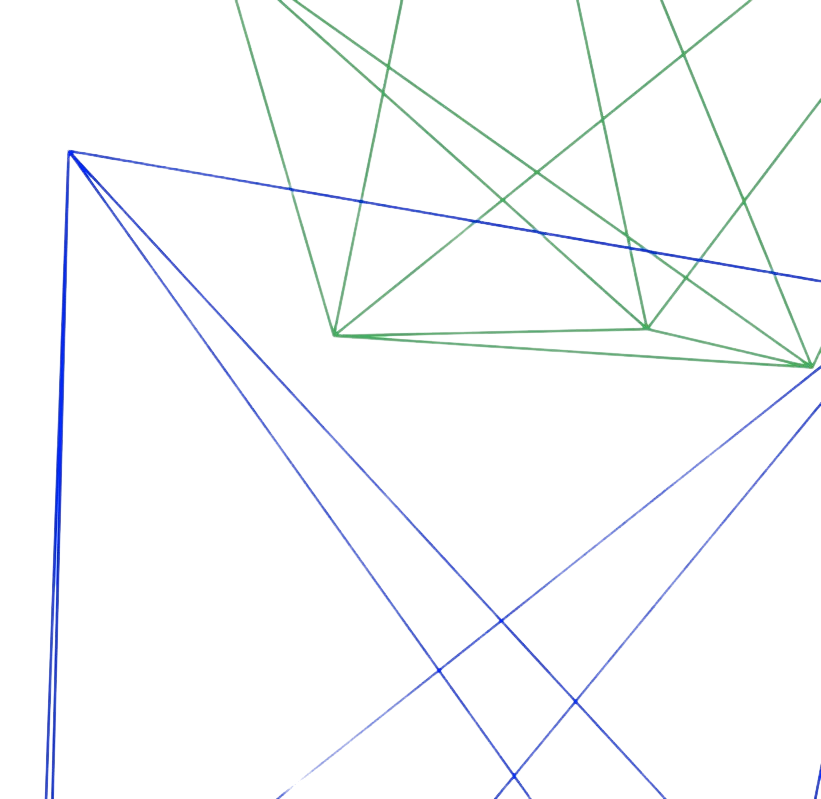
\includegraphics[width=0.5\paperwidth,height=\paperheight]{/root/.config/latex-utils/logos/invert1.png}};

        \node[opacity=0.07,inner sep=0pt, anchor=north west] at (current page.north west){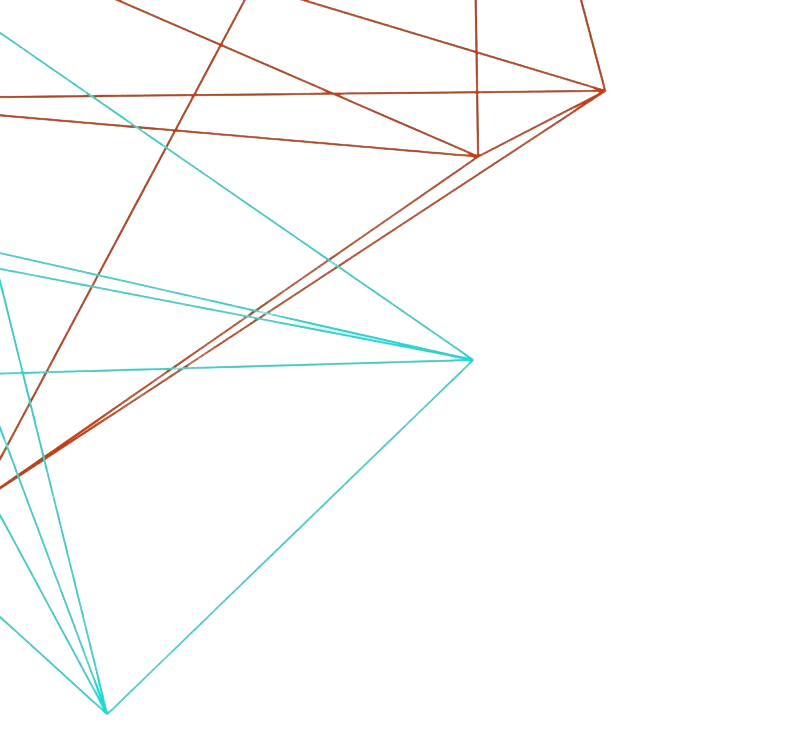
\includegraphics[width=0.5\paperwidth,height=0.5\paperheight]{/root/.config/latex-utils/logos/invert3.png}};




        \node at (page cs:0,0.345) {\Large\textsc{High School Observation and Learning Internship}};
        \node at (page cs:0,0.875) {\Large\bfseries\textsc{Observation Internship}};
        \node at (page cs:0,0.925) {\LARGE\bfseries\textsc{Lycée Français de Barcelone}};

        \node at (page cs:0.5,0) {\Large\textsc{Cyril Lescure - Pedagogical Tutor}};








        %\node[opacity=0.15, inner sep=0pt, anchor=south west] at (current page.south west){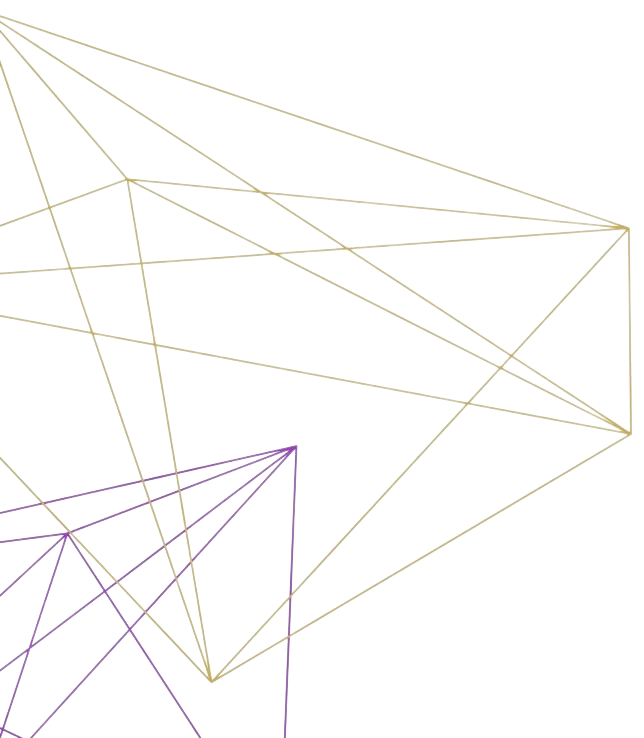
\includegraphics[width=0.5\paperwidth,height=0.5\paperheight]{/root/.config/latex-utils/logos/invert2.png}};

        \node at (page cs:0,0.5) {\fontsize{28}{28.8}\textbf{\ctoptitle}};
        \node at (page cs:0,0.425) {\fontsize{28}{28.8}\textbf{\ctitle}};
        \draw (page cs:0.5,0.375) -- (page cs:-0.5,0.375);
        \node at (page cs:0,0.245) {\LARGE\textsc{\cautor}};
        \node at (page cs:0,0.310) {\Large\textsc{03.06.2019 - 07.06.2019}};


    \end{tikzpicture}
\end{titlepage}


\newgeometry{width=18.625cm, bottom=2cm, top=2cm}

\tikz[remember picture, overlay] \node[opacity=0.3,inner sep=0pt, anchor=north east] at (current page.north east){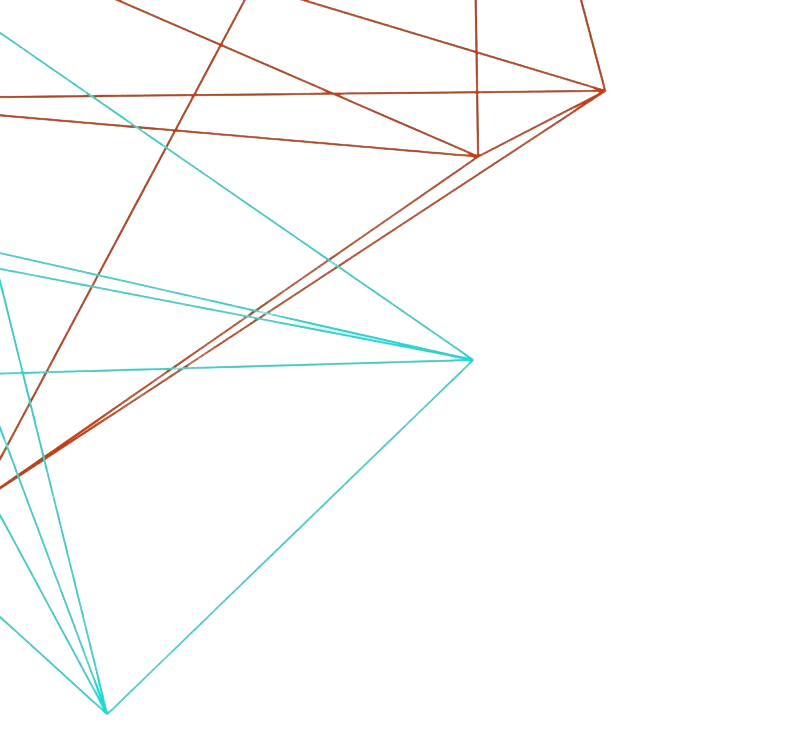
\includegraphics[angle=-90,origin=c,width=0.5\paperheight,height=0.5\paperwidth]{/root/.config/latex-utils/logos/invert3.png}};
\tikz[remember picture,overlay] \node[opacity=0.3,inner sep=0pt, anchor=south east] at (current page.south east){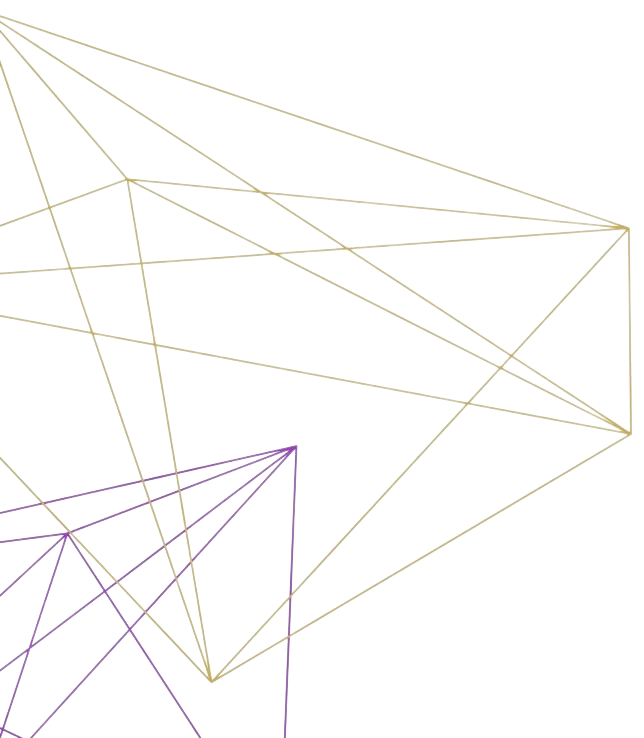
\includegraphics[angle=90,width=0.5\paperwidth,height=0.5\paperheight]{/root/.config/latex-utils/logos/invert2.png}};

\tableofcontents




	
    \newpage

    \section{Introduction}

		Dans ce TP, notre objectif était de concevoir et mettre en œuvre une solution pour compter et identifier efficacement des pièces, en prenant en compte les cas où les pièces se chevauchent. En utilisant une combinaison de techniques traitement d'image, nous avons réussi à développer un système capable de faire face à ces cas pouvant être rencontré dans des application pratiques réelles [Figure 1.1 - Figure 1.2].

		Les techniques employées dans notre approche incluent le filtrage gaussien, la fermeture morphologique, la segmentation et l'étiquetage  pour attribuer des identifiants uniques à chaque pièce. La combinaison de ces méthodes nous a permis de traiter l'image, et de discerner et d'étiqueter avec précision chaque pièce présente dans l'image.
	
    %gg
		\begin{figure}[ht!]
			\begin{floatrow}
				\ffigbox{
					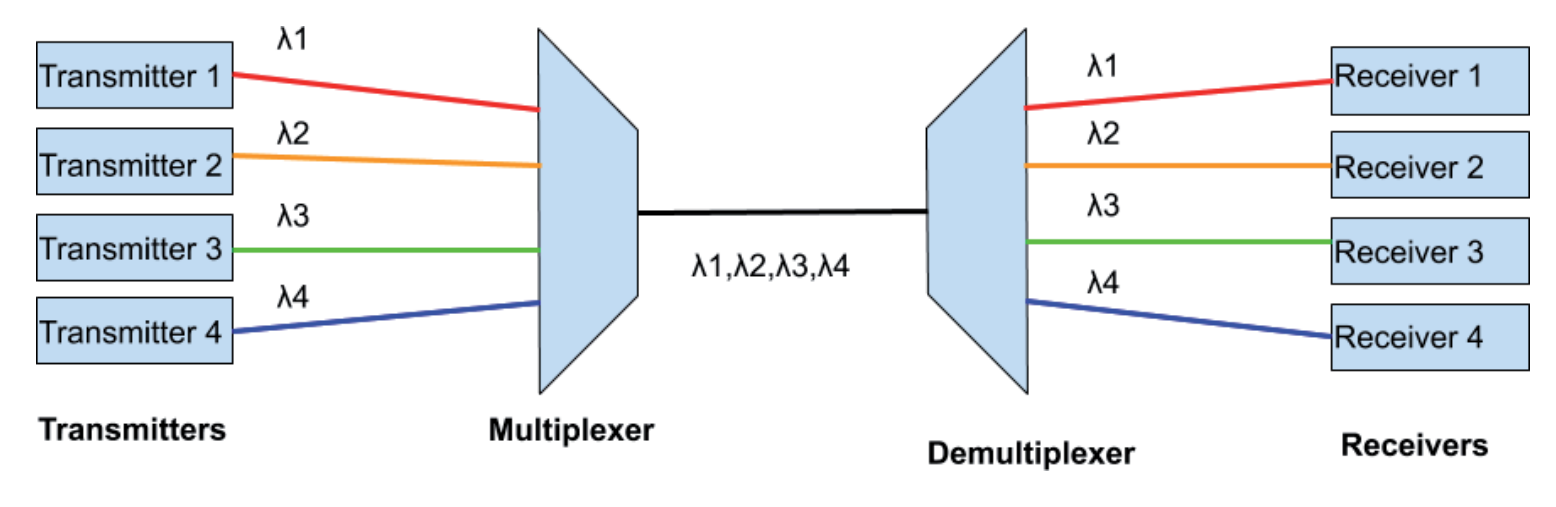
\includegraphics[width=0.3\textwidth]{./object/g1.png}
					\caption{Situation Idéale de distribution}
				}

				\ffigbox{
					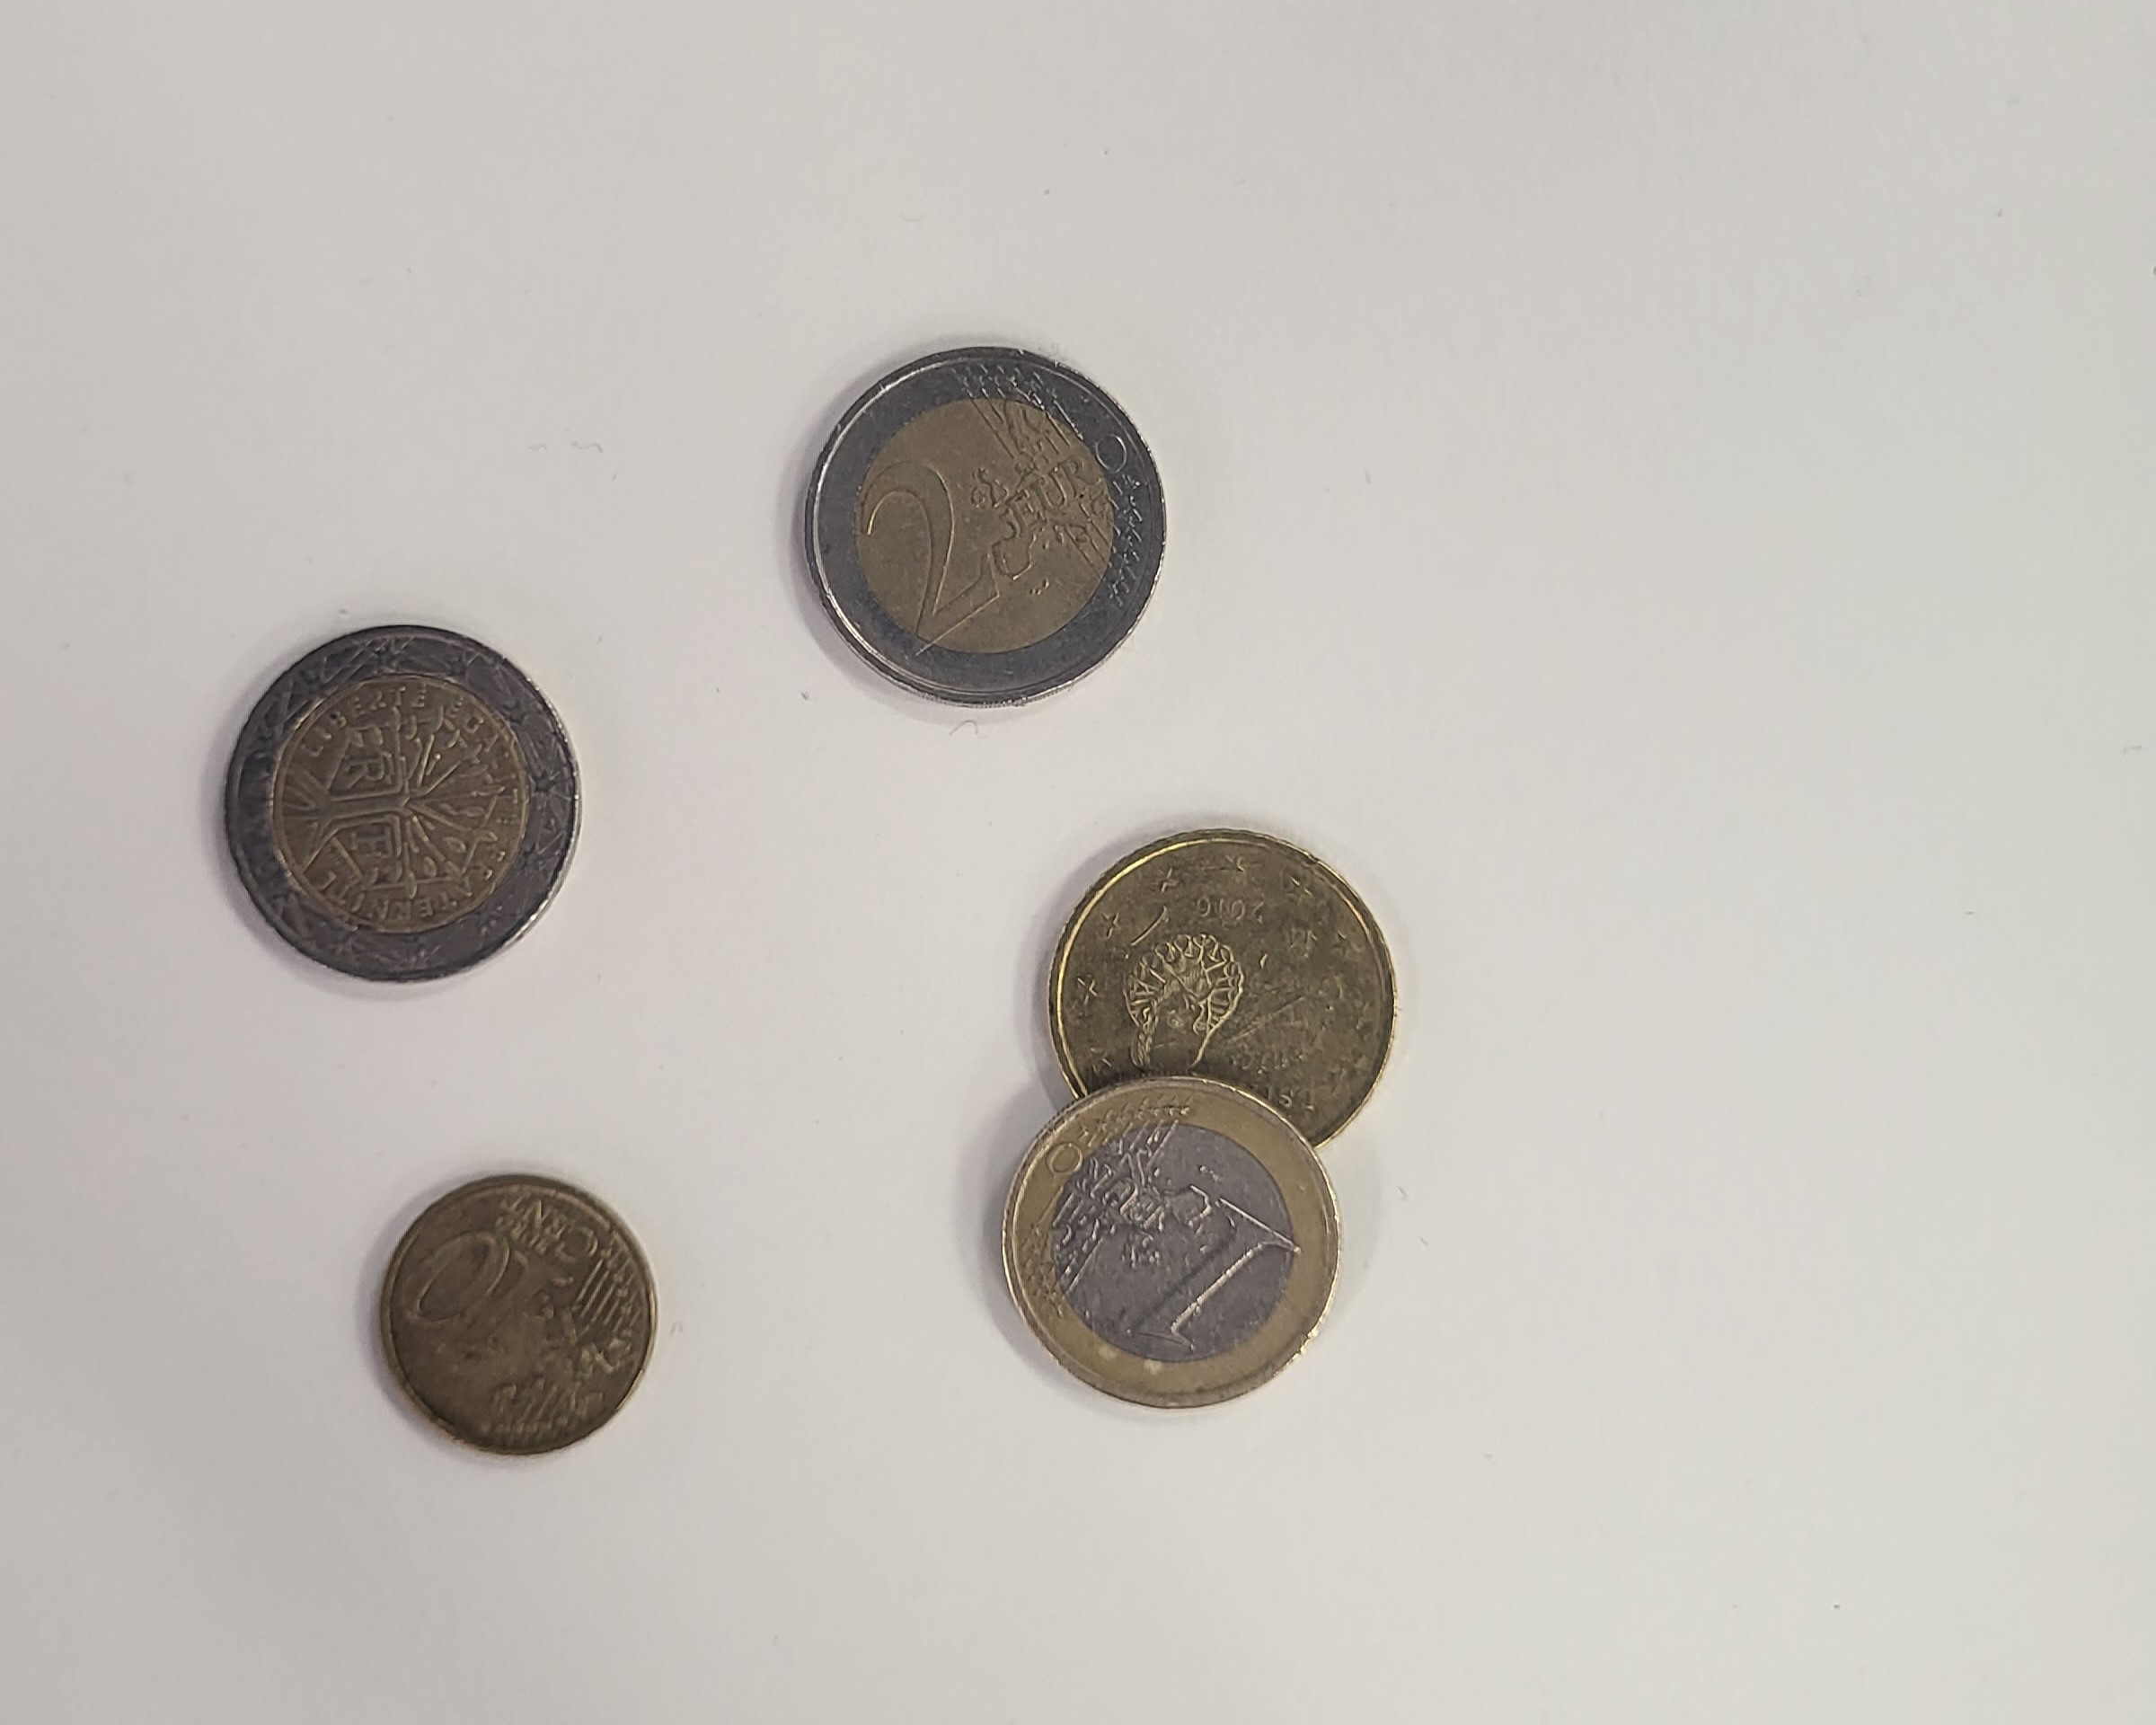
\includegraphics[width=0.3\textwidth]{./object/g2.jpg}
					\caption{Situation particulière réelle}
				}

			\end{floatrow}
		\end{figure}

	\section{Traitement de l'image sous MATLAB}
		
		Dans le but de détecter les différentes pièces contenues dans l'image on aboutira à une segmentation qui nous permettra de traiter chaque pièce séparément et de determiner si elle se superpose, et dans ce cas refaire une segmentation adapté en distinguant les deux pièces superposés.

		De plus, on vise à rendre notre code facilement malléable, nécessitant d'ajuster que 3 paramètres pour traiter l'image correctement:
		\begin{items}[-3pt]{-18pt}{-5pt}
			\item \texttt{correlationThreshold} : le seuil de tolérance pour la determination de la circularité des pièces, permettant à determiner quelles pièces se superposent.
			\item \texttt{closingOrder} : degré de fermeture de l'image pour remplir les parasites éventuels qui peuvent être formé suite à des reflets.
			\item \texttt{objectFilter} : taille maximale des objets a filtrer
		\end{items}
\newpage

		\subsection{Prétraitement}

			Pour commencer avec le traitement de l'image on commence par convertir l'image en niveau de gris en utilisant la fonction \texttt{rgb2gray()} et on redimensionne la taille de l'image à une matrice 255x255 pour effectuer des traitement plus rapides avec la fonction \texttt{imresize()}.
			\begin{figure}[ht!]
				\begin{floatrow}
					\ffigbox{
						\raggedright\texttt{imageFile = imread('g2.jpg');}\\
						\texttt{grayImage= rgb2gray(imageFile);}
						\vspace{0.5cm}

						\texttt{grayImage = imresize(grayImage,[255,255]);}
						\texttt{[sizeIX,sizeIY] = size(grayImage);}
						\vspace{2cm}
					}
					
					\ffigbox{
						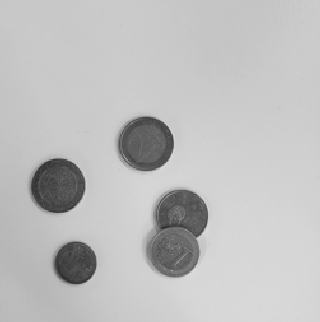
\includegraphics[width=0.3\textwidth]{./object/g3.png}
						\caption{Image en niveau de gris}
					}

				\end{floatrow}
			\end{figure}


		\subsection{Filtrage Gaussien}
			
			Puisque l'on consacre notre projet entièrement à la détection d'objet on fera le choix de prendre un filtre Gaussien plutôt qu'un filtre moyenneur afin the preserver les contours des pièces. De plus la puissance de ce filtre peut-être ajustable ce qui permet un degré de liberté au niveau de la mise au point de l'image. 

			Pour effectuer ce type de filtrage on utilise la propriété dispersive de la distribution gaussienne afin d'appliquer d'appliquer les coefficients appropriés sur un noyau 3x3. On retrouve donc que la Gaussienne en 2 dimension pour notre noyau s'exprime : 
			\begin{equation*}
				\ds{G\left(x,y  \right) =\frac{1}{2\pi\sigma^2}e^{-\frac{x^2+y^2}{2\sigma^2}}}
			\end{equation*}
			On nomme donc les coefficients du noyaux comme étant : 
			\begin{lstlisting}
				c1 = (4*pi*Strength^2);
				c2 = (8*pi*Strength^2);
				c3 = (16*pi*Strength^2);	
			\end{lstlisting}
			Cependant pour éviter d'éclaircir l'image en appliquant ce filtre pour des valeurs de \texttt{Strength} on veut que la somme de tout ces coefficients soient égaux à 1. On va donc effectuer une normalisation: 
			\begin{lstlisting}
				coef_sum = 4 / c3 + 4 / c2 + 1 / c1;
				c1 = c1 / coef_sum;
				c2 = c2 / coef_sum;
				c3 = c3 / coef_sum;
			\end{lstlisting}
			Maintenant il ne manque plus qu'à trouver la valeur optimale pour le traitement d'image. En faisant varier le facteur de puissance \texttt{Strength} de 0.3 à 0.8 par pas de 0.05. 
			On applique donc le filtre pour chaque valeur de \texttt{Strength}, et on effectue un seuillage optimal en utilisant la fonction \texttt{graythresh()} qui renvoi la valeur du seuil entre 0 et 1.

\begin{lstlisting}
	for i = 2:sizeIX-1
    	for j = 2:sizeIY-1
	      imageAverage(i,j) = grayImage(i-1,j-1)/c3 + grayImage(i+1,j-1)/c3 + ...
	      grayImage(i-1,+1)/c3 + grayImage(i+1,j+1)/c3+ ...
	      grayImage(i+1,j)/c2 + grayImage(i-1,j)/c2 + ... 
	      grayImage(i,j+1)/c2 + grayImage(i,j-1)/c2 + ...
	      grayImage(i,j)/c1;
	    end
	  end
\end{lstlisting}
			Pour maintenant mesurer la qualité de l'image ainsi que la différence de qualité avant et après seuillage, on va s'intéresser à la fonction \texttt{edges()} qui nous permet de trouver les contours des objets de l'image. Dans le but d'avoir une image seuillé optimale, on fait la différence de ces deux contours pour pourvoir determiner si les objets dans l'image on été effacé ou pas lors de l'étape de seuillage.
			\begin{lstlisting}
		first_edges = edge(grayImage,'Canny');
  		Threshold = 255*graythresh(imageAverage);

  		imageThreshold = uint8(255*(imageAverage<Threshold));
  		second_edges = edge(imageThreshold,'canny');
  		edge_diff= sum(abs((first_edges(:) - second_edges(:))));
			\end{lstlisting}	
			On conserve alors la valeur de \texttt{Strength} pour laquelle cette différence entre les contours est minimale dans la variable \texttt{best\_strength}, assurant ainsi que le seuillage n'efface pas les objets de l'image filtré.
			\begin{lstlisting}
		if edge_diff < best_edge_diff 
    		  best_strength = averagingStrength;
        	  best_edge_diff = edge_diff;
  		end 
			\end{lstlisting}
			Avec la valeur optimale de puissance pour le filtre Gaussien on effectue un dernier filtrage en prenant \texttt{best\_strength} pour s'assurer que le seuillage de l'image conserve tout les objets dans l'image le résultat étant montré dans la figure ci-dessous. 
			\begin{figure}[ht!]
				\begin{floatrow}
					\ffigbox{
						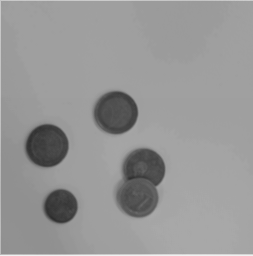
\includegraphics[width=0.35\textwidth]{./object/g5.png}
						\caption{Image optimale du filtre Gaussien}
					}

					\ffigbox{
						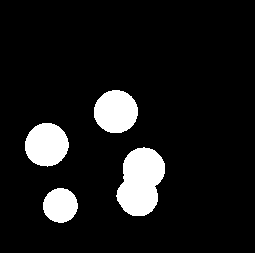
\includegraphics[width=0.35\textwidth]{./object/g4.png}
						\caption{Image seuillé}
					}

				\end{floatrow}
			\end{figure}	
		
			\newpage

		\subsection{Fermeture Morphologique de l'image}

			Dans le cas éventuel qu'il y a des parasites à l'intérieur de l'image on effectue une fermeture 
			en applicant premièrement une dilatation puis une erosion de l'image. Pour pouvoir contrôler la puissance de la fermeture on nomme une variable \texttt{closingOrder} qui determine le nombre de fois à répéter la fermeture.
			\begin{lstlisting}
% Dilatation de l'image
imageDilation = imageThreshold;
  imageDilationOrder = imageThreshold;

  for n = 1:closingOrder
    for i = 2:sizeIX-1
      for j = 2:sizeIY-1
        if(imageDilationOrder(i,j) == 0 )
          if(imageDilationOrder(i-1,j) == 255 || ..
  	    imageDilationOrder(i+1,j) == 255 || ...
            imageDilationOrder(i,j-1) == 255 || ...
	    imageDilationOrder(i,j+1) == 255)
            imageDilation(i,j) = uint8(255);
          end
        end
      end
    end
    imageDilationOrder = imageDilation;
  end

  % Erosion de l'image

  imageErosion = imageDilation;
  imageErosionOrder = imageThreshold; % image recursive pour l'ordre de fermeture

  for n = 1:closingOrder
    for i = 2:sizeIX-1
      for j = 2:sizeIY-1
        if(imageErosionOrder(i,j) == 0 )
          if(imageErosionOrder(i-1,j) == 255 || ...
  	  imageErosionOrder(i+1,j) == 255 || ...
          imageErosionOrder(i,j-1) == 255 || ...
  	  imageErosionOrder(i,j+1) == 255)
            imageErosion(i,j) = uint8(255);
          end
        end
      end
    end
    imageErosionOrder = imageErosion;
  end

imageClosing = imageErosion;
			\end{lstlisting}

		\subsection{Segmentation et Étiquetage}
			
			Après avoir réalisé la fermeture morphologique on fait une segmentation en 4 étapes puis on liste toutes les objets détectés en utilisant leur étiquette  et on filtre les objets qui ne sont pas des pièces un applicant un seuil de taille \texttt{objectFilter}
			\begin{lstlisting}
		objectFilter=200;
		for k=1:254
		  label = sum(sum(imageSegmented == k));
  		  if label > objectFilter
  		    listObjects(k)= label;
  		  end
		end
		obj_number = nnz(listObjects); %Nombre d'objets
		labelObject = (find(listObjects)); %Etiquetttes objets
			\end{lstlisting}

			\begin{figure}[ht!]
				\centering
				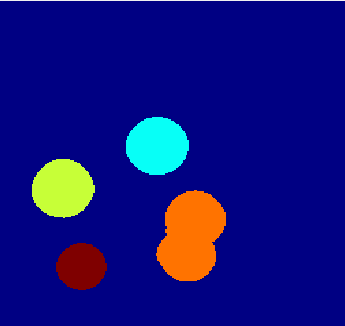
\includegraphics[width=0.3\textwidth]{./object/g10.png}
				\caption{Image segmentée}
			\end{figure}
			Après avoir segmenté et étiquetter les objects il faut maintenant determiner si certaines pièces sont l'une par dessus l'autre. Pour ceci on se propose de mesurer la circularité de chaque objet en utilisant la fonction \texttt{regionprops()} qui permet de retourner des information sur chaque objet. \\
			Grâce à celle-ci on récupère les coordonnées des centre géométrique de chaque objet ainsi que leur circularité et leur aire. Dans le cas ou l'objet n'est pas un disque parfait alors la circularité s'écarte de 1, en applicant un seuil pour la tolérance de la circularité on distingue ainsi quels objets sont des pièces qui se superposent.
			\begin{lstlisting}
      superpose = 0;
      for k=1:obj_number
        areaObject(k) = sum(sum(imageSegmented == labelObject(k)));
        Objects(k) = regionprops((imageSegmented == labelObject(k)), ...
            "Circularity","Centroid", "Area");
        Radius(k) = sqrt(Objects(k).Area) /pi 
        if Objects(k).Circularity < correlationThreshold
          display(sprintf(['Il y a une superposition de deux pieces '...
              'voir la piece : %i\n'],k))
          superpose = 1;
        end
      end
			\end{lstlisting}

		\subsection{Séparation des pièces}
			
			On cherche ensuite à séparer les pièces qui se superposent en utilisant la fonction \texttt{imfindcircles} qui permet d'identifier les cercles dans l'image et de retourner leur rayon ainsi que leur centre. 
			\begin{lstlisting}
	min_radius = uint8(min(Radius)) ;
	max_radius = uint8(max(Radius)) + 10;
	edges_img = edge(imageSegmented,'canny');

	[centers, radii] = imfindcircles(edges_img, [min_radius, max_radius],...
	  'ObjectPolarity', 'bright', 'Sensitivity', 0.9025);
			\end{lstlisting}

			Grâce à ces donnés on peut alors dessiner sur une nouvelle grille de taille 255x255 les pièces détectées en utilisant la fonction \texttt{meshgrid()} et en applicant le mask de chaque pièce par dessus:
			\begin{lstlisting}
    segmented_img = zeros(size(grayImage));

    num_circles = size(centers, 1);
     for i = 1:num_circles
         center = centers(i, :);
         radius = radii(i);
         [X, Y] = meshgrid(1:size(grayImage, 2), 1:size(grayImage, 1));
    
         circle_mask = ((X - center(1)).^2 + (Y - center(2)).^2) <= radius^2;
    
         segmented_img(circle_mask) = i;
     end
			\end{lstlisting}

			On obtient alors l'image suivante : 
			\begin{figure}[ht!]
				\centering
				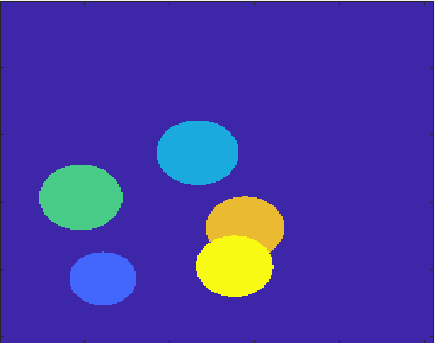
\includegraphics[width=0.3\textwidth]{./object/g6.png}
				\caption{Séparation des pièces}
			\end{figure}

			On finit alors le traitement par ajouter du texte sur chaque pièce:
			\begin{lstlisting}
     for k=1:num_circles
         text(centers(k,1),centers(k,2),['Coin ', num2str(k)], ...
          'HorizontalAlignment', 'center', 'FontSize',8);
     end
			\end{lstlisting}

			\begin{figure}[ht!]
				\centering
				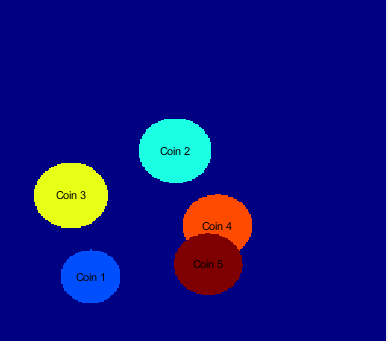
\includegraphics[width=0.3\textwidth]{./object/g7.png}
				\caption{Pieces séparés et différentiés}
			\end{figure}

\section{Annexe}

Code MATLAB (UTF-8):

\begin{lstlisting}
clear all;
close all;

%% --  Valeurs a configurer --
correlationThreshold = 0.925 % Seuil de tolerance de la circularite
closingOrder = 1 % ordre de la fermeture configurable

%% -- Pretraitement
% Recuperation de l'image et adaptation de taille
imageFile = imread('g3.jpg');
grayImage= rgb2gray(imageFile);

grayImage = imresize(grayImage,[255,255]);
[sizeIX,sizeIY] = size(grayImage);

% Filtrage par filtre Gaussien 3x3
imageAverage = grayImage;

%% -- Filtrage Gaussien --
% Coefficients gaussiens

best_edge_diff = Inf;

for Strength = 0.35:0.05:0.8
c1 = (4*pi*Strength^2);
c2 = (8*pi*Strength^2);
c3 = (16*pi*Strength^2);

% Normalisation des coefficients
total_sum = 4 / c3 + 4 / c2 + 1 / c1;
c1 = c1 / total_sum;
c2 = c2 / total_sum;
c3 = c3 / total_sum;

 for i = 2:sizeIX-1
    for j = 2:sizeIY-1
      imageAverage(i,j) = grayImage(i-1,j-1)/c3 + grayImage(i+1,j-1)/c3 + ...
      grayImage(i-1,+1)/c3 + grayImage(i+1,j+1)/c3+ ...
      grayImage(i+1,j)/c2 + grayImage(i-1,j)/c2 + ...
      grayImage(i,j+1)/c2 + grayImage(i,j-1)/c2 + ...
      grayImage(i,j)/c1;
    end
  end

  first_edges = edge(grayImage,'Canny');
  % Seuillage de limage
  Threshold = 255*graythresh(imageAverage);

  imageThreshold = uint8(255*(imageAverage<Threshold));
  second_edges = edge(imageThreshold,'canny');
  edge_diff= sum(abs((first_edges(:) - second_edges(:))));

  if edge_diff < best_edge_diff 
        best_strength = Strength;
        best_edge_diff = edge_diff;
  end 

end

c1 = (4*pi*best_strength^2);
c2 = (8*pi*best_strength^2);
c3 = (16*pi*best_strength^2);

% Normalisation des coefficients
total_sum = 4 / c3 + 4 / c2 + 1 / c1;
c1 = c1 / total_sum;
c2 = c2 / total_sum;
c3 = c3 / total_sum;

 for i = 2:sizeIX-1
    for j = 2:sizeIY-1
      imageAverage(i,j) = grayImage(i-1,j-1)/c3 + grayImage(i+1,j-1)/c3 + ...
      grayImage(i-1,+1)/c3 + grayImage(i+1,j+1)/c3+ ...
      grayImage(i+1,j)/c2 + grayImage(i-1,j)/c2 + ...
      grayImage(i,j+1)/c2 + grayImage(i,j-1)/c2 + ...
      grayImage(i,j)/c1;
    end
 end


imageAverage = uint8(imageAverage);

% Adaptation du seuillage par technique d'Otsu
Threshold = 255*graythresh(imageAverage);

% Seuillage de l'image
imageThreshold = uint8(255*(imageAverage<Threshold));

%% -- Fermeture de l'image --
  % Dilatation de l'image
  imageDilation = imageThreshold;
  imageDilationOrder = imageThreshold; % image recursive pour l'ordre de dilatation

  for n = 1:closingOrder
    for i = 2:sizeIX-1
      for j = 2:sizeIY-1
        if(imageDilationOrder(i,j) == 0 )
          if(imageDilationOrder(i-1,j) == 255 || ...
             imageDilationOrder(i+1,j) == 255 || ...
             imageDilationOrder(i,j-1) == 255 || ...
             imageDilationOrder(i,j+1) == 255)
            imageDilation(i,j) = uint8(255);
          end
        end
      end
    end
    imageDilationOrder = imageDilation;
  end	

  
  % Erosion de l'image

  imageErosion = imageDilation;
  imageErosionOrder = imageThreshold; % image recursive pour l'ordre de fermeture

  for n = 1:closingOrder
    for i = 2:sizeIX-1
      for j = 2:sizeIY-1
        if(imageErosionOrder(i,j) == 0 )
          if(imageErosionOrder(i-1,j) == 255 || ...
             imageErosionOrder(i+1,j) == 255 || ...
             imageErosionOrder(i,j-1) == 255 || ...
             imageErosionOrder(i,j+1) == 255)
            imageErosion(i,j) = uint8(255);
          end
        end
      end
    end
    imageErosionOrder = imageErosion;
  end

imageClosing = imageErosion;

%% -- Segmentation -- 

imageSegmented = imageClosing;
label_init=60;
label = label_init;


% Premiere passe : depart en haut a gauche
for i = 2:sizeIX
  for j = 2:sizeIY
    if (imageSegmented(i,j) > 0)
      if (imageSegmented(i-1,j) == 0 && imageSegmented(i,j-1) == 0)
        imageSegmented(i,j) = label ;
        label = label + 2 ;
      else
        if (imageSegmented(i-1,j) > 0 && imageSegmented(i,j-1) > 0)
          imageSegmented(i,j) = min([imageSegmented(i-1,j), ...
              imageSegmented(i,j-1)]) ;
        elseif (imageSegmented(i-1,j) > 0 && imageSegmented(i,j-1) == 0)
          imageSegmented(i,j) = imageSegmented(i-1,j) ;
        else
          imageSegmented(i,j) = imageSegmented(i,j-1) ;
        end
      end
    end
  end
end



% Deuxieme passe : depart en haut a droite
for i = 2:sizeIX
  for j = sizeIY-1:-1:1
    if (imageSegmented(i,j) > 0)
      if (imageSegmented(i-1,j) > 0 && imageSegmented(i,j+1) > 0)
        imageSegmented(i,j) = min([imageSegmented(i,j), ...
            imageSegmented(i-1,j), imageSegmented(i,j+1)]);
      elseif (imageSegmented(i-1,j) > 0 && imageSegmented(i,j+1) == 0)
        imageSegmented(i,j) = min([imageSegmented(i,j), imageSegmented(i-1,j)]);
      elseif (imageSegmented(i-1,j) == 0 && imageSegmented(i,j+1) > 0)
        imageSegmented(i,j) = min([imageSegmented(i,j), imageSegmented(i,j+1)]);
      end
    end
  end
end


%Troisieme passe : depart en bas a droite
for i = sizeIX-1:-1:1
  for j = sizeIY-1:-1:1
    if (imageSegmented(i,j) > 0)
      if (imageSegmented(i+1,j) > 0 && imageSegmented(i,j+1) > 0)
        imageSegmented(i,j) = min([imageSegmented(i,j), ...
            imageSegmented(i+1,j), imageSegmented(i,j+1)]);
      elseif (imageSegmented(i+1,j) > 0 && imageSegmented(i,j+1) == 0)
        imageSegmented(i,j) = min([imageSegmented(i,j), imageSegmented(i+1,j)]);
      elseif (imageSegmented(i+1,j) == 0 && imageSegmented(i,j+1) > 0)
        imageSegmented(i,j) = min([imageSegmented(i,j), imageSegmented(i,j+1)]);
      end
    end
  end
end

% Quatrieme passe : depart en bas a gauche
for i = sizeIX-1:-1:1
  for j = 2:sizeIY
    if (imageSegmented(i,j) > 0)
      if (imageSegmented(i+1,j) > 0 && imageSegmented(i,j-1) > 0)
        imageSegmented(i,j) = min([imageSegmented(i,j), ...
            imageSegmented(i+1,j), imageSegmented(i,j-1)]);
      elseif (imageSegmented(i+1,j) > 0 && imageSegmented(i,j-1) == 0)
        imageSegmented(i,j) = min([imageSegmented(i,j), imageSegmented(i+1,j)]);
      elseif (imageSegmented(i-1,j) == 0 && imageSegmented(i,j-1) > 0)
        imageSegmented(i,j) = min([imageSegmented(i,j), imageSegmented(i,j-1)]);
      end
    end
  end
end


% On reunit dans une liste 1x254 les differents objets trouves
objectFilter = 200
for k=1:254
  label = sum(sum(imageSegmented == k));
  if label > objectFilter
  listObjects(k)= label;
  end
end

% Affichage du nombre d'objets listes
obj_number = nnz(listObjects);


% Etiquetage des objets en recuperant leur valeur de la liste
labelObject = (find(listObjects))

%Calcul de l'aire reelle et l'aire du contour de chaque objets


superpose = 0;
count = 0;
for k=1:obj_number
  areaObject(k) = sum(sum(imageSegmented == labelObject(k)));
  Objects(k) = regionprops((imageSegmented == labelObject(k)), ...
      "Circularity","Centroid", "Area");
  Radius(k) = sqrt(Objects(k).Area) /pi ;
  if Objects(k).Circularity < correlationThreshold
    display(sprintf(['Il y a une superposition de deux pieces '...
        'voir la piece : %i\n'],k+count));
    count = count +1;
    superpose = 1;
  end
end

min_radius = uint8(min(Radius)) ;
max_radius = uint8(max(Radius)) + 10;
edges_img = edge(imageSegmented,'canny');

[centers, radii] = imfindcircles(edges_img, [min_radius, max_radius], ...
    'ObjectPolarity', 'bright', 'Sensitivity', 0.9025);

% Differentiation
segmented_img = zeros(size(grayImage));

num_circles = size(centers, 1);
for i = 1:num_circles
    center = centers(i, :);
    radius = radii(i);
    [X, Y] = meshgrid(1:size(grayImage, 2), 1:size(grayImage, 1));
    
    circle_mask = ((X - center(1)).^2 + (Y - center(2)).^2) <= radius^2;
    
    segmented_img(circle_mask) = i;
end


if superpose == 0
  disp('Aucune piece ne se superpose, le nombre de pieces est donc :')
  disp(num_circles)
else
  disp(sprintf(['Le nombre de pieces est : %i'],num_circles));
end


figure(3);subplot(1,2,1);imhist(imageAverage);
figure(3);subplot(1,2,2);imhist(grayImage);

figure(1); subplot(2,3,2);imshow(imageAverage);title('Averaged')
figure(1);subplot(2,3,1);imshow(grayImage);title('Grayed')
figure(1);subplot(2,3,3);imshow(imageThreshold);title('Thresholded')
figure(1);subplot(2,3,4);imshow(imageDilation);title('Dilated')
figure(1);subplot(2,3,5);imshow(imageClosing);title('Closing')
figure(1);subplot(2,3,6);imagesc(imageSegmented);axis off; 
colormap('jet'); colorbar; title('Segmented');
figure(2);imagesc(segmented_img);axis off; 
colormap('jet'); colorbar; title('Result');

sort_centers = sortrows(centers, 2);
for k=1:num_circles
    text(sort_centers(k,1),sort_centers(k,2),['Coin ', num2str(k)], ...
     'HorizontalAlignment', 'center', 'FontSize',8);
end

\end{lstlisting}

\begin{figure}[ht!]
	\begin{floatrow}
		\ffigbox{
			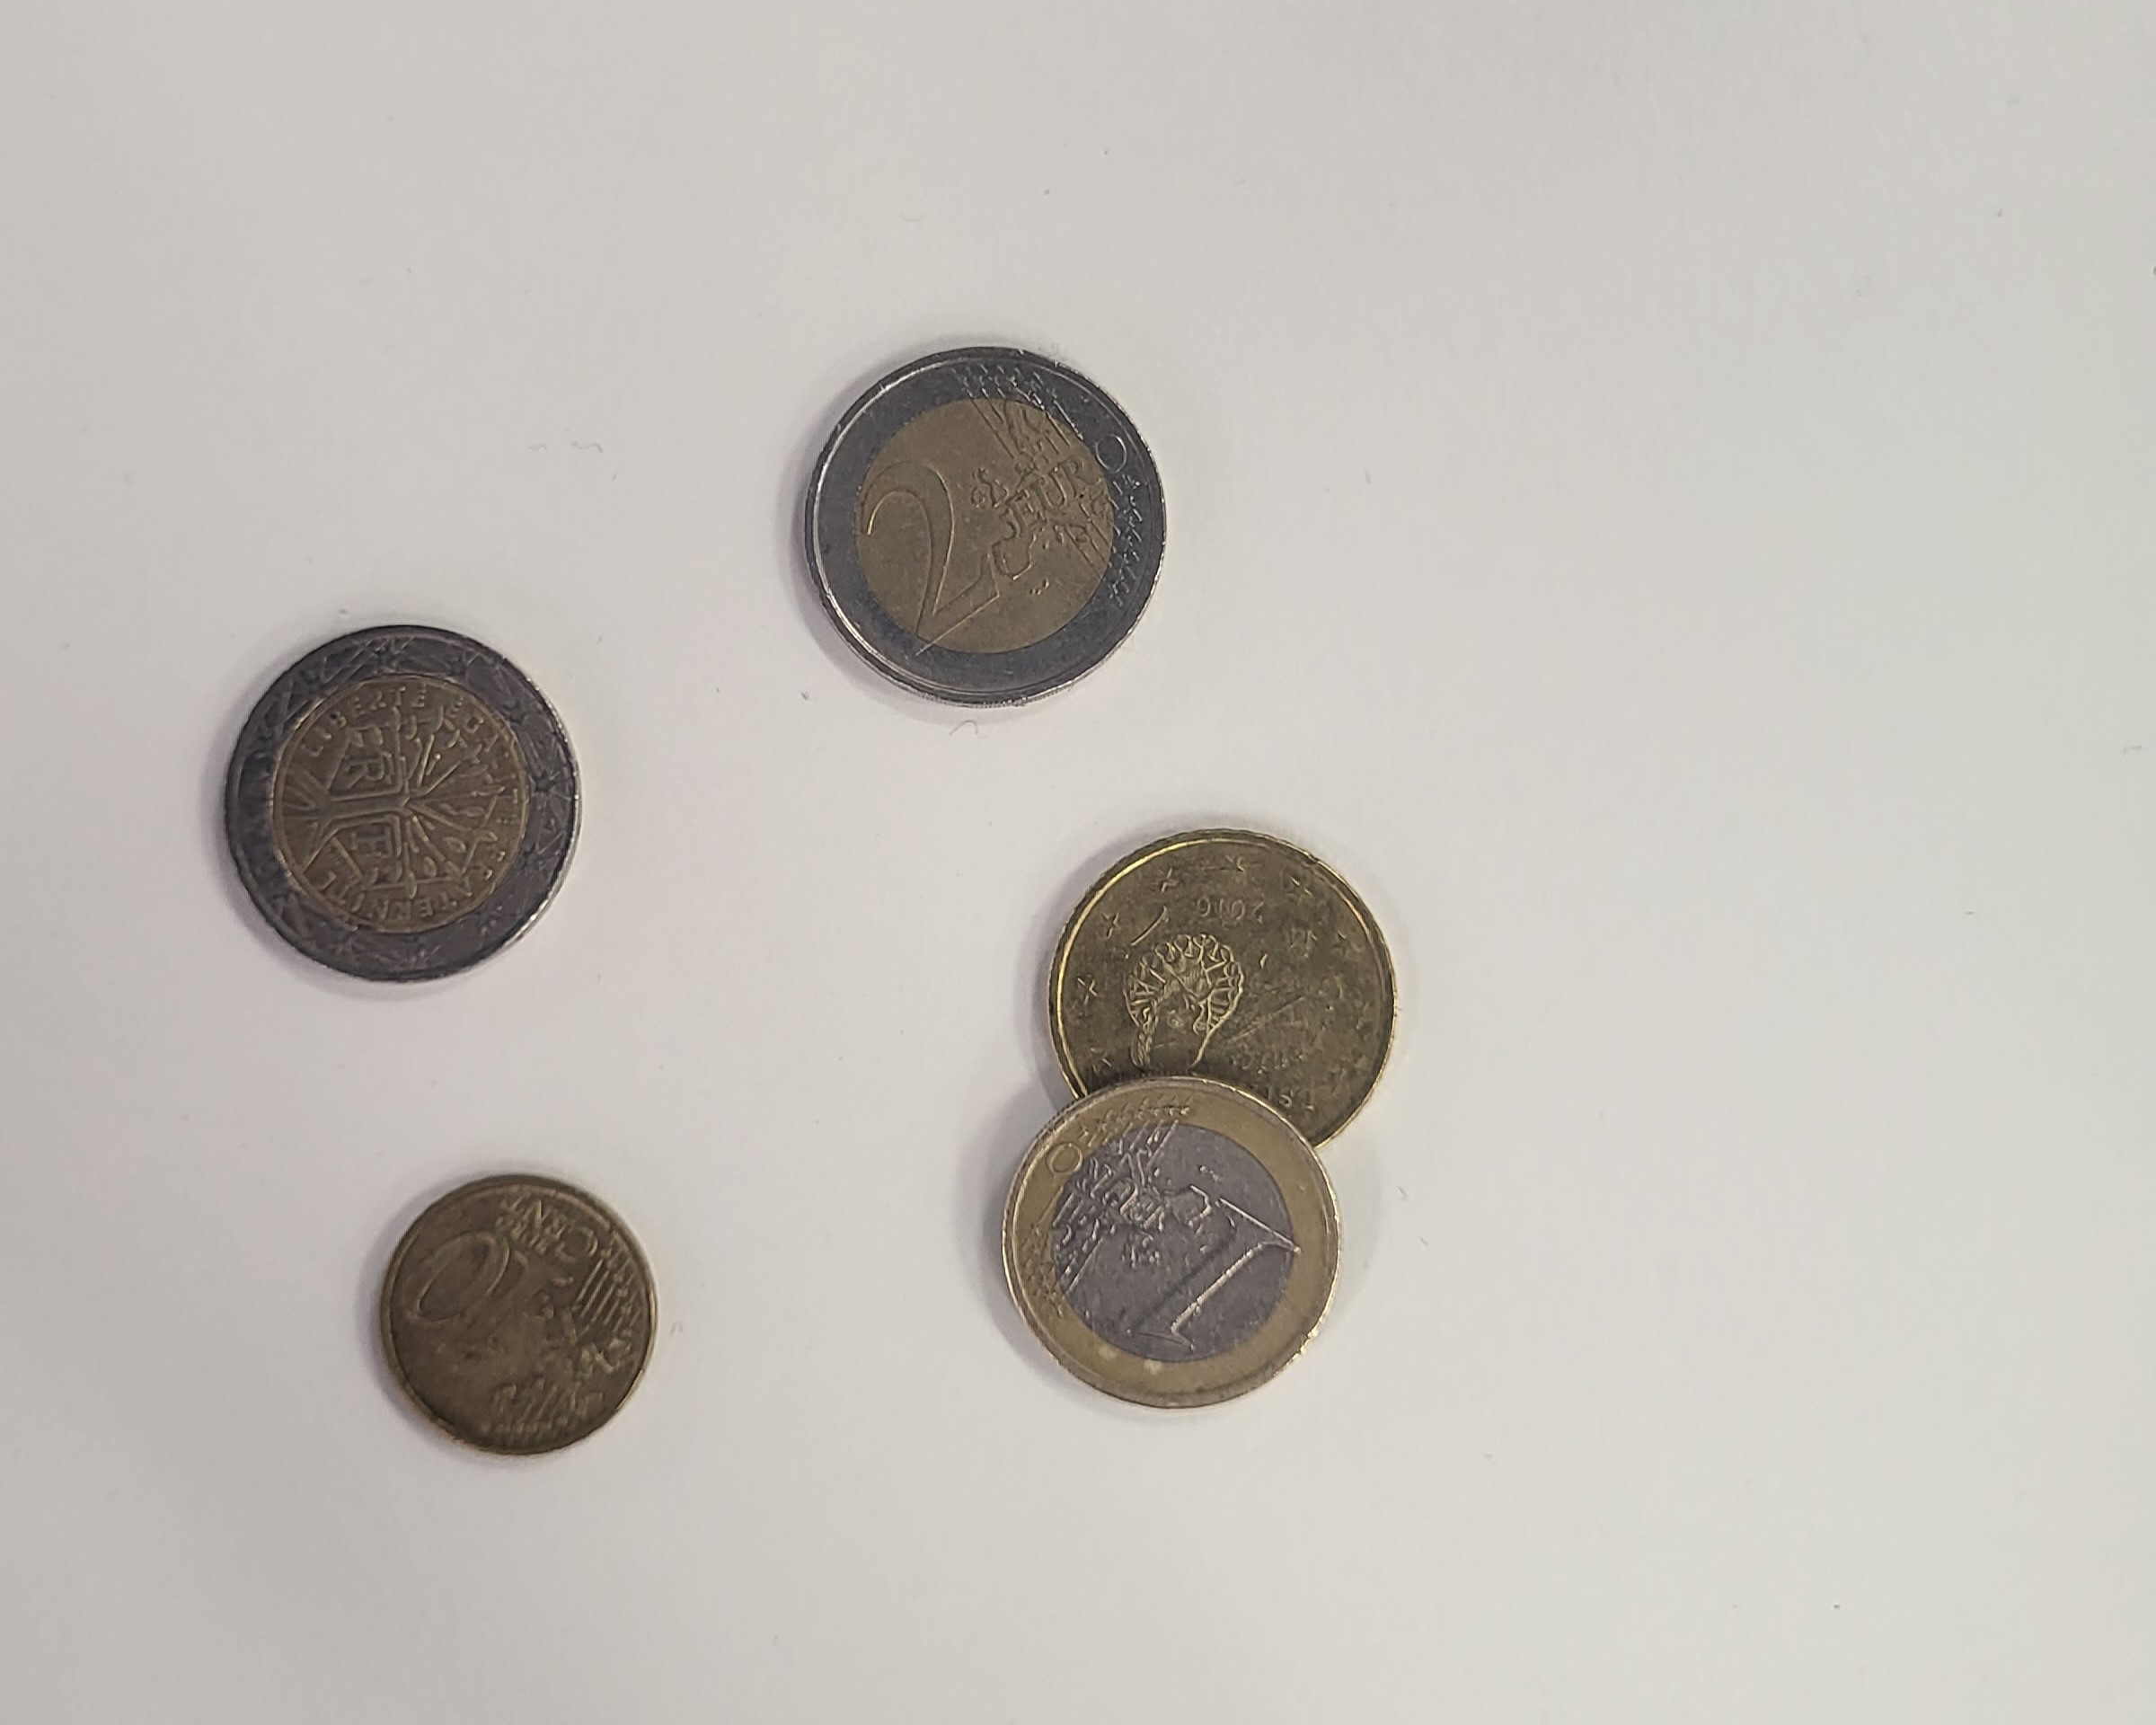
\includegraphics[width=0.35\textwidth]{./object/g2.jpg}
			\caption{Image pré-traitement}
		}
		
		\ffigbox{
			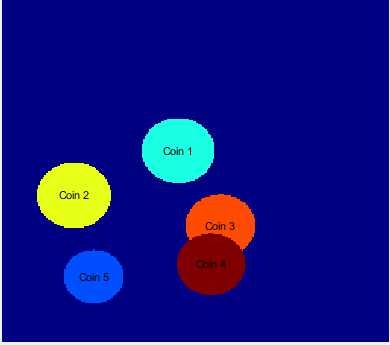
\includegraphics[width=0.35\textwidth]{./object/12.png}
			\caption{Image post-traitement}
		}
		
	\end{floatrow}
\end{figure}

\begin{figure}[ht!]
	\begin{floatrow}
		\ffigbox{
			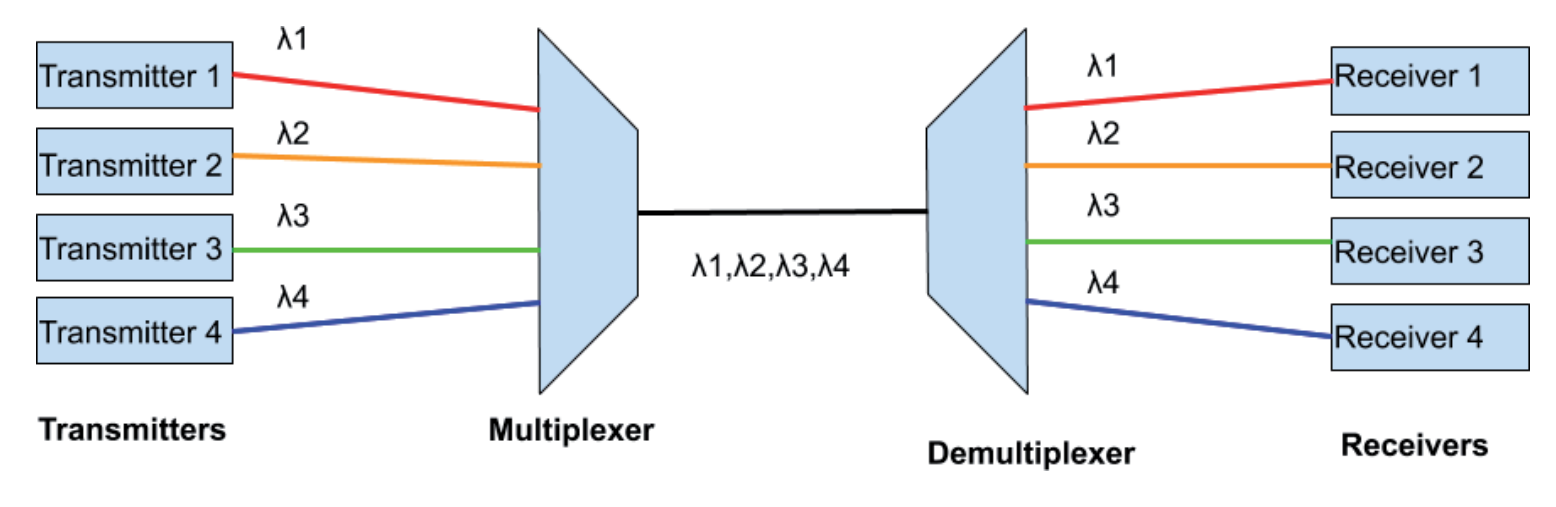
\includegraphics[width=0.35\textwidth]{./object/g1.png}
			\caption{Image pré-traitement (avec ombres)}
		}
		
		\ffigbox{
			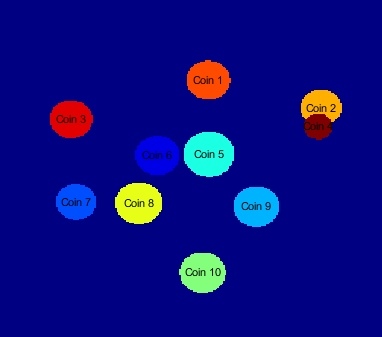
\includegraphics[width=0.35\textwidth]{./object/g22.png}
			\caption{Image post-traitement}
		}
		
	\end{floatrow}
\end{figure}

\begin{figure}[ht!]
	\begin{floatrow}
		\ffigbox{
			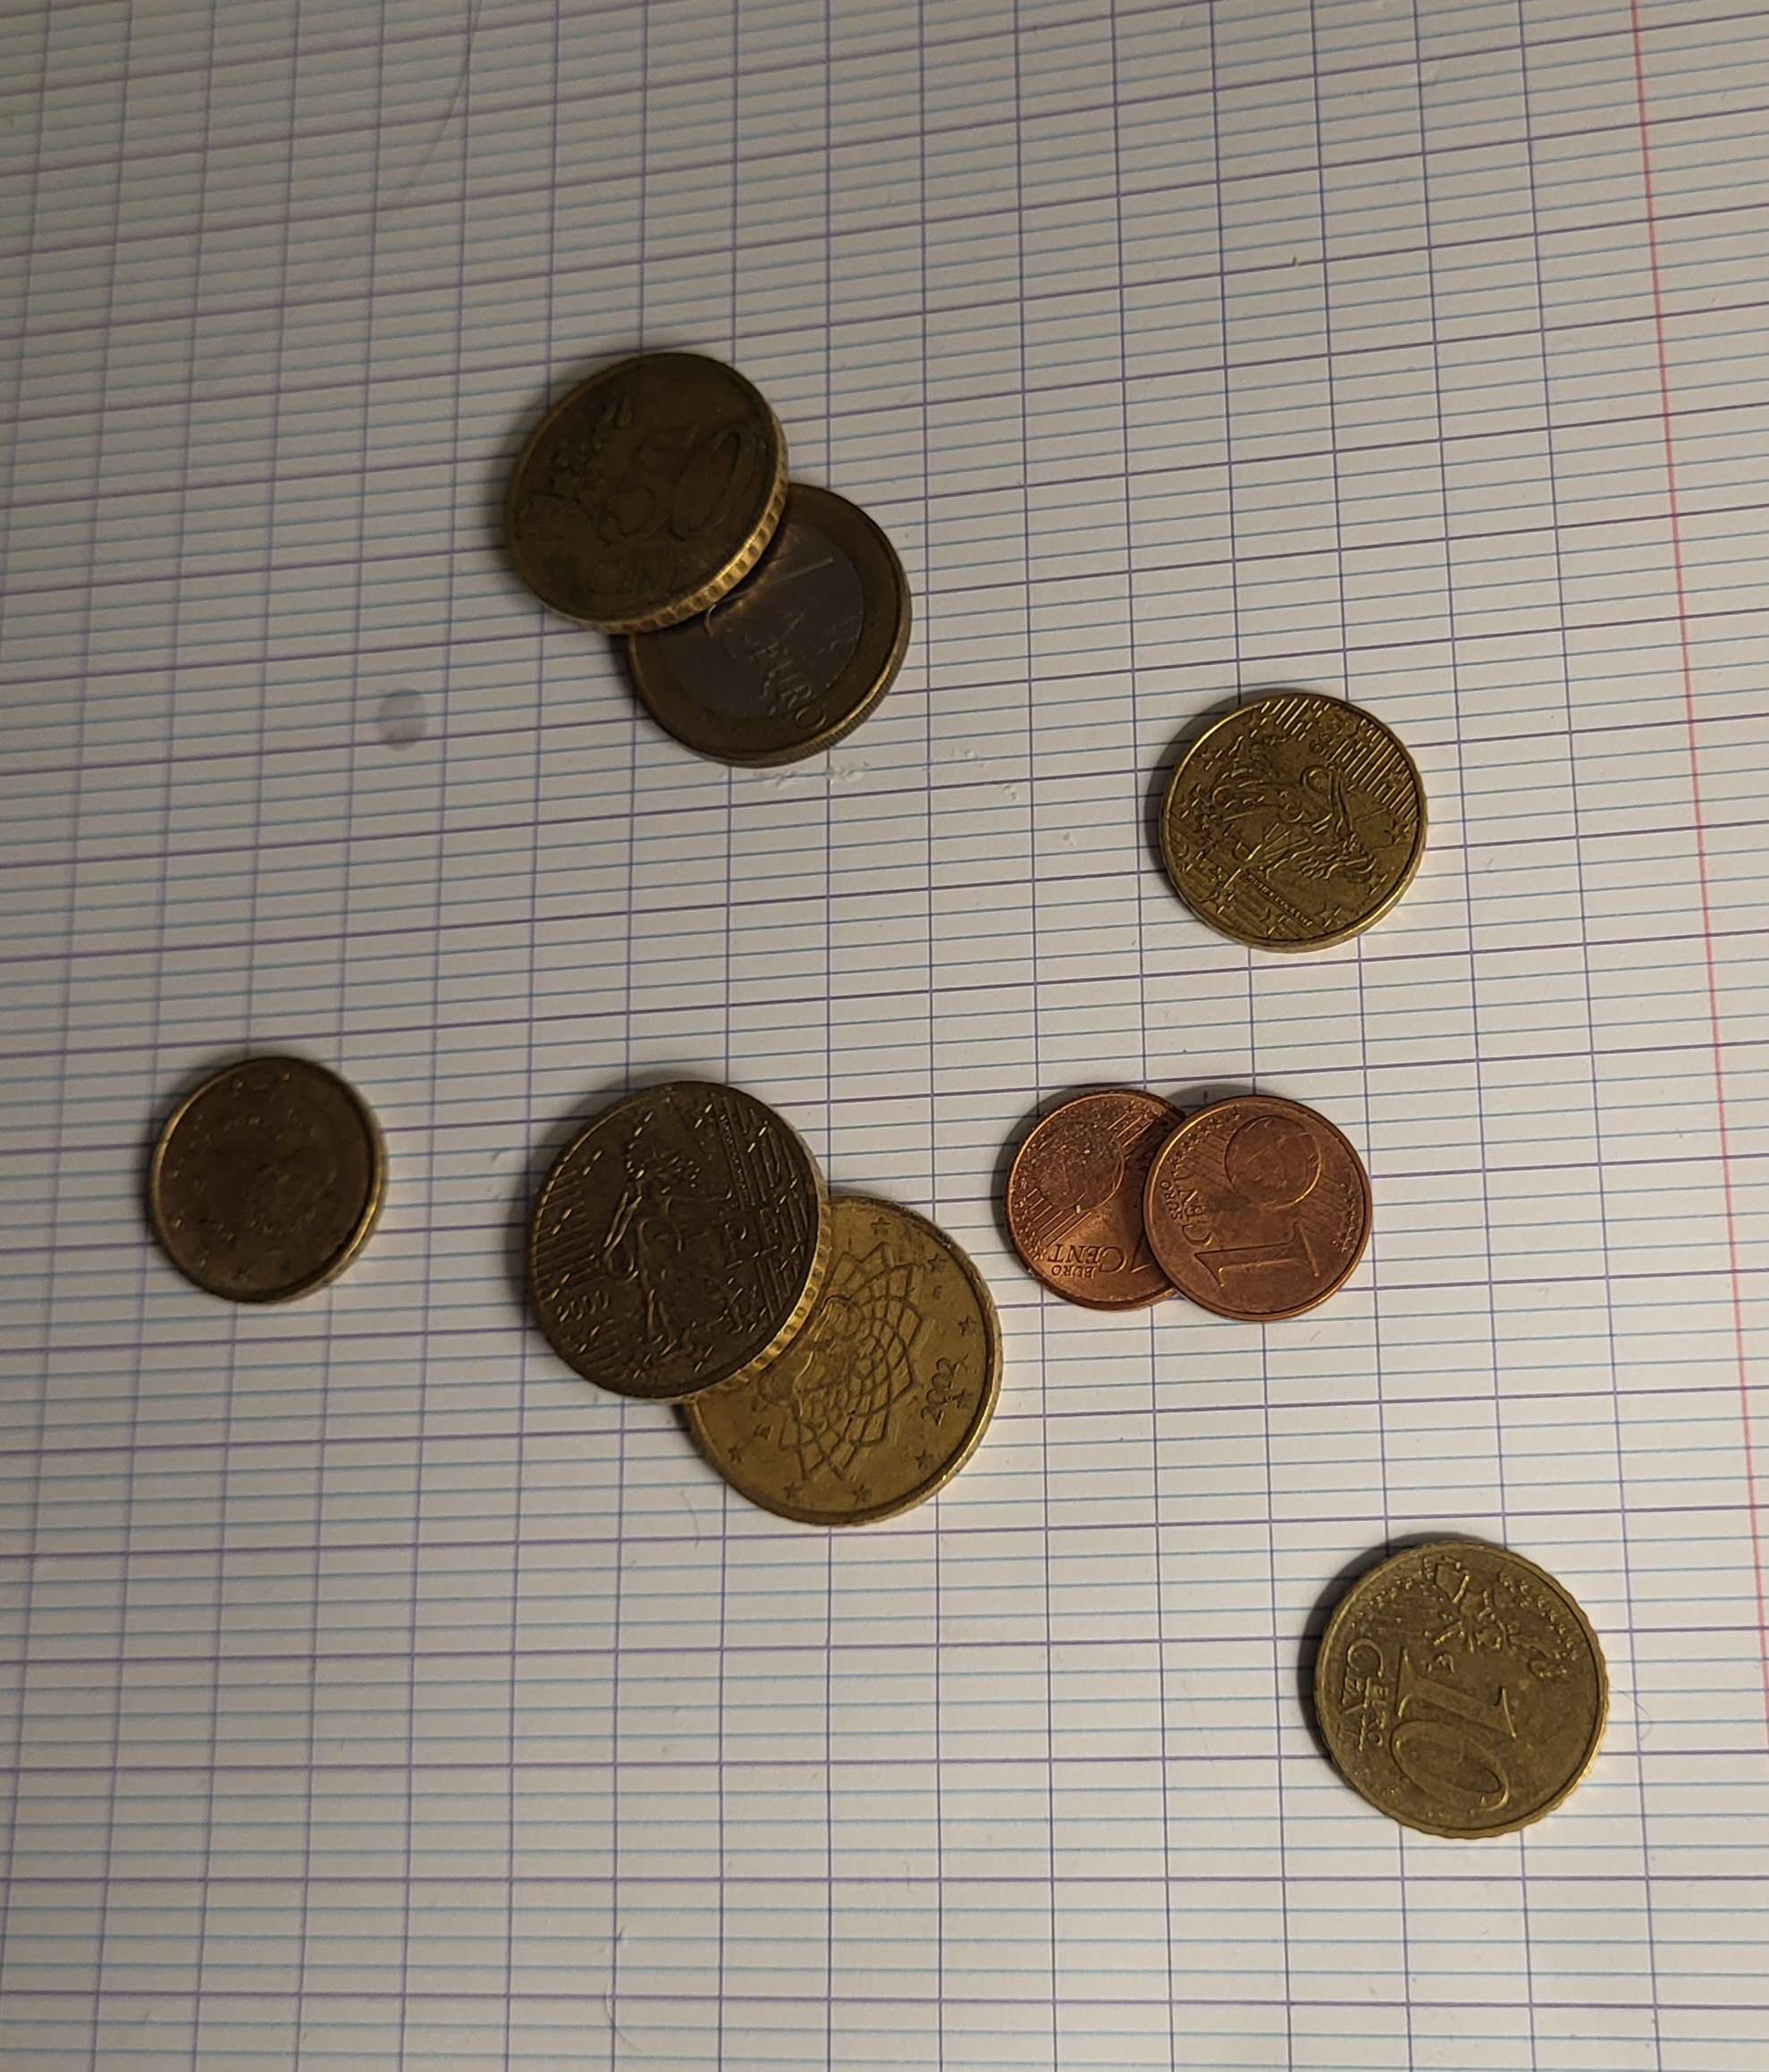
\includegraphics[width=0.35\textwidth]{./object/g3.jpg}
			\caption{Image pré-traitement}
		}
		
		\ffigbox{
			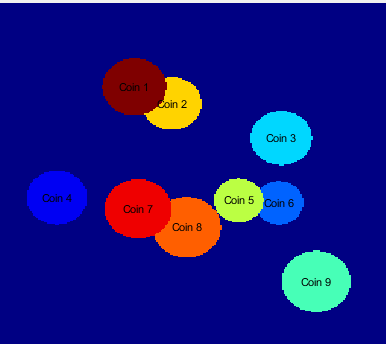
\includegraphics[width=0.35\textwidth]{./object/g32.png}
			\caption{Image post-traitement}
		}
		
	\end{floatrow}
\end{figure}


		







			
	

	


	

\end{document}
